\documentclass[12pt, Draft, onecolumn]{IEEEtran}

\usepackage[cmex10]{amsmath}
\usepackage{amsthm,amssymb}
\usepackage{algorithmicx}
\usepackage{graphicx, epsfig, color}
\usepackage{array}
\usepackage{cite}
\usepackage{mathabx}

\def\ie{{\it i.e., }}
\def\etc{{\it etc}}
\def\adhoc{{\it ad hoc }}
\def\eg{{\it e.g. }}
\def\iid{{\it i.i.d. }}

\DeclareMathOperator*{\argmin}{arg\,min}
\DeclareMathOperator*{\argmax}{arg\,max}
\DeclareMathOperator*{\skw}{skew}
\DeclareMathOperator*{\dist}{d}
\DeclareMathOperator*{\tr}{tr}
\DeclareMathOperator*{\re}{Re}
\DeclareMathOperator*{\im}{Im}
\DeclareMathOperator*{\E}{E}
\DeclareMathOperator*{\prob}{\mathbb{P}}

\def\diff{{\mathrm{d}}}
\def\ba{{\mathbf{a}}}
\def\bd{{\mathbf{d}}}
\def\be{{\mathbf{e}}}
\def\bff{{\mathbf{f}}}
\def\bg{{\mathbf{g}}}
\def\bh{{\mathbf{h}}}
\def\bm{{\mathbf{m}}}
\def\bn{{\mathbf{n}}}
\def\bq{{\mathbf{q}}}
\def\br{{\mathbf{r}}}
\def\bs{{\mathbf{s}}}
\def\bt{{\mathbf{t}}}
\def\bu{{\mathbf{u}}}
\def\bv{{\mathbf{v}}}
\def\bw{{\mathbf{w}}}
\def\bx{{\mathbf{x}}}
\def\by{{\mathbf{y}}}
\def\bz{{\mathbf{z}}}


\def\bA{{\mathbf{A}}}
\def\bB{{\mathbf{B}}}
\def\bC{{\mathbf{C}}}
\def\bF{{\mathbf{F}}}
\def\bG{{\mathbf{G}}}
\def\bH{{\mathbf{H}}}
\def\bI{{\mathbf{I}}}
\def\bK{{\mathbf{K}}}
\def\bN{{\mathbf{N}}}
\def\bR{{\mathbf{R}}}
\def\bS{{\mathbf{S}}}
\def\bT{{\mathbf{T}}}
\def\bU{{\mathbf{U}}}
\def\bV{{\mathbf{V}}}
\def\bW{{\mathbf{W}}}
\def\bX{{\mathbf{X}}}
\def\bY{{\mathbf{Y}}}
\def\bZ{{\mathbf{Z}}}

\def\calC{{\mathcal{C}}}
\def\calE{{\mathcal{E}}}
\def\calH{{\mathcal{H}}}
\def\calM{{\mathcal{M}}}
\def\calS{{\mathcal{S}}}
\def\calU{{\mathcal{U}}}
\def\calX{{\mathcal{X}}}
\def\calY{{\mathcal{Y}}}
\def\calZ{{\mathcal{Z}}}
\def\calT{{\mathcal{T}}}

\newtheorem{theorem}{Theorem}
\newtheorem{lemma}{Lemma}
\newtheorem{definition}{Definition}

\begin{document}
\title{Proof of the Converse}
\author{Pang-Chang Lan}
\maketitle

\section{Problem Statement and Assumptions}
Let's consider a discrete memoryless wiretap channel with perfect CSIT but no CSIRE as shown in Fig. \ref{fig.secrecy_noCSIR_channel}. The perfect CSIT is causally available to the transmitter. That is, the encoder knows $S^i$ before transmission $i$ occurs. Let the message set be $\calM=\{1,2,\cdots,2^{nR}\}$. A $(2^{nR},n)$ code is used for this setup. The encoder performs $x_i(m,s^i)$ for $i\in [1:n]$, and the decoder performs $\hat{m}(y^n)$. Note that the function $x_i(\cdot, \cdot)$ is deterministic and fixed before the transmission begins.

\begin{figure}[h]
\centering
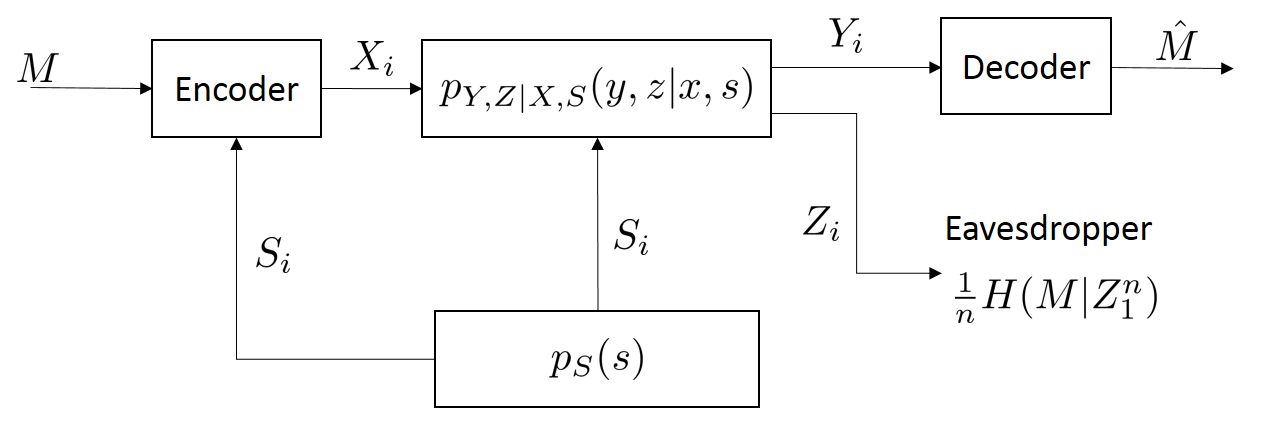
\includegraphics[scale=.6]{figs/secrecy_noCSIR_channel}
\caption{Discrete memoryless wiretap channel with perfect CSIT but no CSIRE}
\label{fig.secrecy_noCSIR_channel}
\end{figure}

\section{Main Theorem}
\begin{theorem}
Suppose that the main channel is less noisy than the wiretap channel, \ie $I(U;Y)\geq I(U;Z)$ for all $U$ such that $(U,S)\rightarrow (X,S)\rightarrow (Y,Z)$ forms a Markov chain. The secrecy capacity of the discrete memoryless wiretap channel with perfect CSIT but no CSIRE is given by
\begin{equation}
C_s = \max_{p(u)t(u,s),p(x|t,s)} I(T;Y)-I(T;Z)
\end{equation}
where $T$ is the auxiliary random variables independent of $S$ and satisfying the Markov relation $T\rightarrow (X,S)\rightarrow (Y,Z)$, the cadinality bound is $|\calT|\leq \min\{(|\calX|-1)|\calS|+1,|\calY|\}$, and $x:\calT\times\calS\rightarrow\calX$ is a deterministic function.
\end{theorem}

\section{Achievability Proof}
We first prove that the following rate is achievable in general, namely,
\begin{equation}\label{eq.achievable}
R_s = \max_{p(u)p(t|u),x(t,s)} I(U;Y)-I(U;Z)
\end{equation}
where $U$ and $T$ are auxiliary random variables independent of $S$ and satisfying the Markov relation $U\rightarrow T\rightarrow (X,S)\rightarrow (Y,Z)$, the cadinality bound is given by $|\calU|\leq |\calT|$.

We use multicoding and a three-step randomized encoding scheme.\\

\noindent {\bf Codebook generation.} For each message $m\in \calM$, generate a subcodebook $\calC(m)$ consisting of $2^{n(\tilde{R}-R)}$ sequences $u^n(l)$ for $l\in [(m-1)2^{n(\tilde{R}-R)}+1:m2^{n(\tilde{R}-R)}]$ which is randomly and independently generated according to the distribution $\prod_{i=1}^n p_U(u_i)$. This codebook is revealed to all the nodes.\\

\noindent {\bf Encoding.} To send message $m\in\calM$, the encoder uniformly randomly chooses an index $L$ from $\calC(m)$. Then it generates $t^n(L)$ by random coding according to the distribution $\prod_{i=1}^n p_{T|U}(t_i|u_i(l))$. The channel input at time $i$ is then given by $x_i=x(t_i(L),s_i)$ where $x(\cdot,\cdot)$ is a deterministic function.\\

\noindent {\bf Decoding.} Given $Y^n=y^n$, find the unique $\hat{m}$ such that $(u^n(l), y^n)\in\calT^n_{\varepsilon}(U,Y)$ for some $u^n(l)\in\calC(\hat{m})$.\\

\noindent {\bf Analysis.} By code translation, we can obtain an equivalent wiretap channel described by
\begin{align*}
p_{Y,Z|T}(y,z|t) &= \sum_{x\in\calX, s\in\calS}P_{Y,Z,X,S|T}(y,z,x,s|t)\\
&= \sum_{x\in\calX, s\in\calS}P_{Y,Z|X,T,S}(y,z|x,t,s)p_{X|T,S}(x|t,s)p_{S|T}(s|t)\\
&= \sum_{x\in\calX, s\in\calS}P_{Y,Z|X}(y,z|x)\delta_K(x=x(t,s))p_{S}(s)\\
&= \sum_{s\in\calS}P_{Y,Z|X}(y,z|x(t,s))p_{S}(s).
\end{align*}
The resulting equivalent DMC without CSI is shown in Figure \ref{fig.secrecy_noCSIR_channel_equivalent}.
\begin{figure}[h]
\centering
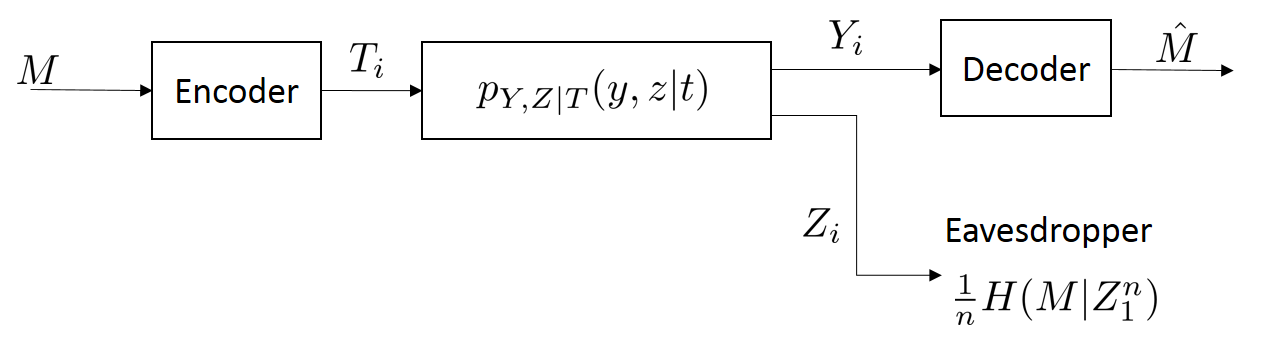
\includegraphics[scale=.6]{figs/secrecy_noCSIR_channel_equivalent}
\caption{Equivalent discrete memoryless wiretap channel with no CSI}
\label{fig.secrecy_noCSIR_channel_equivalent}
\end{figure}
The rest of the analysis procedure follows that of the wiretap channel.

Let $M$ be the transmitted message and $L$ be the randomly picked index within codebook $\calC(M)$. Let $\calE$ be the event of error decoding. Let $\calE_1=\{(U^n(l), Y^n)\notin\calT^n_{\varepsilon}(U,Y) \text{ for all $U^n(l)\in \calC(m)$}\}$ and $\calE_2=\{(U^n(l), Y^n)\in\calT^n_{\varepsilon}(U,Y) \text{ for some $l\neq L$}\}$. Then
\begin{align*}
P(\calE)\leq P(\calE_1\cup\calE_2) \leq P(\calE_1)+P(\calE_2)
\end{align*}
By LLN, $P(\calE_1)\rightarrow 0$ as $n\rightarrow \infty$. By the packing lemma, $P(\calE_2)\rightarrow 0$ as $n\rightarrow \infty$ if $\tilde{R}<I(U;Y)-\delta(\varepsilon)$. Hence, the error probability diminishes as $n$ goes to infinity.

By following the proof in the Network Information Theory book, the equivocation at the eavesdropper can also be shown to approach $0$ as $n\rightarrow \infty$ if $\tilde{R}-R\geq I(U;Z)$. Hence, the achievable rate follows as \eqref{eq.achievable}.

Now, by the less noisy property, we have
\begin{align}
R_s &= \max_{p(u)p(t|u),x(t,s)} I(U;Y)-I(U;Z)\notag\\
&= \max_{p(u)p(t|u),x(t,s)} I(T,U;Y)-I(T,U;Z)-(I(T;Y|U)-I(T;Z|U))\notag\\
&= \max_{p(t),x(t,s)} I(T;Y)-I(T;Z)
\end{align}
where the last equality follows since $I(T;Y|U)-I(T;Z|U)\geq 0$ and by letting $U=T$, it is made $0$. Hence, the achievability follows.

\section{Converse Proof}
%To prove the converse, we first assume that the wiretap channel is less noisy, \ie $I(U;Y)\geq I(U;Z)$ for all $P_UP_{X|U}$ such that $(U,S)\rightarrow (X,S)\rightarrow (Y,Z)$.

Suppose there exists a code such that $R_e\leq \varepsilon_n$ where $\varepsilon_n\rightarrow 0$ as $n\rightarrow \infty$. Note that by Fano's inequality, $H(M|Y^n)\leq n\varepsilon_n'$ where $\varepsilon_n'\rightarrow 0$ as $n\rightarrow \infty$. We have
\begin{align}
nR_s &= H(M)-H(M|Y^n) +H(M|Y^n)\notag\\
&\leq I(M;Y^n) + n\varepsilon_n'\notag\\
&= I(M;Y^n)-I(M;Z^n) +nR_e+n\varepsilon_n'\notag\\
&\leq  I(M;Y^n)-I(M;Z^n) +n(\varepsilon_n'+\varepsilon_n)\notag\\
&= \sum_{i=1}^n \left[I(M;Y_i|Y_1^{i-1})-I(M;Z_i|Z_{i+1}^n)\right]+n(\varepsilon_n'+\varepsilon_n)\notag\\
&= \sum_{i=1}^n \left[I(M,Z_{i+1}^n;Y_i|Y_1^{i-1})-I(Z_{i+1}^n;Y_i|Y_1^{i-1},M)-I(M,Y_1^{i-1};Z_i|Z_{i+1}^n)+I(Y_1^{i-1};Z_i|Z_{i+1}^n,M)\right]\notag\\
&\quad+n(\varepsilon_n'+\varepsilon_n)\notag\\
\label{eq.sum_ineq1}
&= \sum_{i=1}^n \left[I(M,Z_{i+1}^n;Y_i|Y_1^{i-1})-I(M,Y_1^{i-1};Z_i|Z_{i+1}^n)\right]+n(\varepsilon_n'+\varepsilon_n)\\
&= \sum_{i=1}^n \left[I(M;Y_i|Y_1^{i-1},Z_{i+1}^n)+I(Z_{i+1}^n;Y_i|Y_1^{i-1})-I(M;Z_i|Z_{i+1}^n,Y_1^{i-1})-I(Y_1^{i-1};Z_i|Z_{i+1}^n)\right]\notag\\
&\quad+n(\varepsilon_n'+\varepsilon_n)\notag\\
\label{eq.sum_ineq2}
&= \sum_{i=1}^n \left[I(M;Y_i|Y_1^{i-1},Z_{i+1}^n)-I(M;Z_i|Y_1^{i-1},Z_{i+1}^n)\right]+n(\varepsilon_n'+\varepsilon_n)\\
\label{eq.first_outcome}
&= \sum_{i=1}^n \left[I(T_i;Y_i|V_i)-I(T_i;Z_i|V_i)\right]+n(\varepsilon_n'+\varepsilon_n)
\end{align}
where \eqref{eq.sum_ineq1} and \eqref{eq.sum_ineq2} are due to Csiszar sum identity, and in \eqref{eq.first_outcome} auxiliary random variables $V_i = (Y_1^{i-1},Z_{i+1}^n)$ and $T_i = (M,V_i)$ are introduced such that $(V_i,S_i)\rightarrow (T_i,S_i)\rightarrow (X_i,S_i)  \rightarrow (Y_i,Z_i)$ forms a Markov chain. Note that here $V_i$ and $T_i$ are dependent on $S_i$.

%Now, by the less noisy property, we have
%\begin{align}
%I(\tilde{U}_i;Y_i|V_i)-I(\tilde{U}_i;Z_i|V_i)
%\end{align}

Hence,
\begin{align}
\eqref{eq.first_outcome}
\label{eq.time_sharing}
&= \left[I(T_Q;Y_Q|V_Q,Q)-I(T_Q;Z_Q|V_Q,Q)\right]+n(\varepsilon_n'+\varepsilon_n)\\
\label{eq.after_time_sharing}
&= \left[I(T;Y|V)-I(T;Z|V)\right]+n(\varepsilon_n'+\varepsilon_n)\\
&\leq \max_v \left[I(T;Y|V=v)-I(T;Z|V=v)\right]+n(\varepsilon_n'+\varepsilon_n)\notag\\
\label{eq.C_s}
&= n\max_{p(t|s)p(x|t,s)}\left[I(T;Y)-I(T;Z)\right]+n(\varepsilon_n'+\varepsilon_n)\notag\\
&= n\max_{p(u)t(u,s),p(x|t,s)}\left[I(T;Y)-I(T;Z)\right]+n(\varepsilon_n'+\varepsilon_n)
\end{align}
where in \eqref{eq.time_sharing} a time-sharing random variable $Q$ is introduced, \eqref{eq.after_time_sharing} holds by letting $V = (V_Q,Q)$, $U=(U_Q,Q)$, $Y=Y_Q$, and $Z=Z_Q$, \eqref{eq.C_s} is because of the Markov chain $(T,S)\rightarrow (X,S)\rightarrow (Y,Z)$ and the functional representation lemma, and $t(\cdot,\cdot)$ is a deterministic function. 

\begin{lemma}[functional representation]
Let $(S,T,X)\sim p(s,t,x)$. Then $T$ can be represented as a function of $(S,U)$ for some random variable $U$ of cardinality $|\calU|\leq |\calS|(|\calT|-1)+1$ such that $U$ is independent of $S$ and $U\rightarrow (T,S)\rightarrow X$ forms a Markov chain.
\end{lemma}




%\bibliographystyle{IEEEtran}
%\bibliography{security}

\end{document}


